\documentclass[tikz]{standalone}

\begin{document}
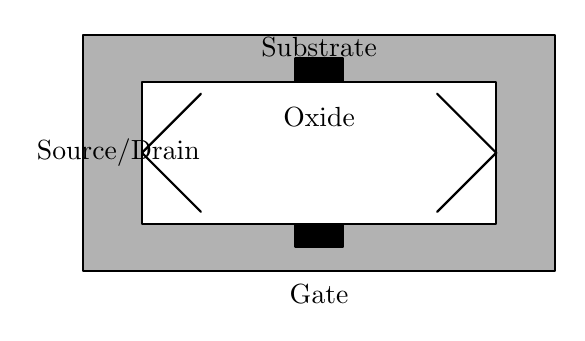
\begin{tikzpicture}[scale=1.5, thick, line cap=round, line join=round]
% Substrate
\draw[fill=black!30] (-2,-1) rectangle (2,1);

% Source/Drain
\draw[fill=black] (-1,-0.5) rectangle (-0.5,0.5);
\draw[fill=black] (1,-0.5) rectangle (0.5,0.5);

% Gate
\draw[fill=black] (-0.2,-0.8) rectangle (0.2,0.8);

% Oxide
\draw[fill=white] (-1.5,-0.6) rectangle (1.5,0.6);

% Connections
\draw (-1.5,0) -- (-1,-0.5);
\draw (-1.5,0) -- (-1,0.5);
\draw (1.5,0) -- (1,-0.5);
\draw (1.5,0) -- (1,0.5);

% Labels
\node at (0,0.9) {Substrate};
\node at (0,0.3) {Oxide};
\node at (-1.7,0) {Source/Drain};
\node at (0,-1.2) {Gate};

\end{tikzpicture}
\end{document}